\documentclass[12pt]{beamer}
\usepackage[utf8]{inputenc}
\usepackage{lmodern}
\usepackage{german}
\usetheme{Berkeley}
\title[Kick-Off Semesterarbeit]{Implementation einer Win/Win Strategie für das TSP}
\author{Andreas Brönnimann}
\institute{Hochschule für Technik Zürich}
\date{12.10.2011}

\setbeamerfont{footnote}{size=\tiny}
\setbeamertemplate{footline}[frame number]
\setbeamertemplate{navigation symbols}{}

\begin{document}

    \begin{frame}
        \titlepage
    \end{frame}

    \begin{frame}
        \frametitle{Ablauf}
        \tableofcontents
    \end{frame}

	\section{Ausgangslage}
	\begin{frame}
        \frametitle{Ausgangslage}
		\begin{itemize}
			\item Travelling Salesman Problem	
				\begin{itemize}
					\item metrisches TSP ($\Delta$TSP)
					\item Dreiecksungleichung erfüllt
				\end{itemize}
				\begin{figure}[H]
					\centering
					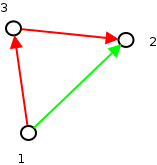
\includegraphics[width=2cm]{gfx/triangle_inequality}
				\end{figure}
				
			\item Win/Win Strategie
				\begin{itemize}
					\item metrisches Travelling Salesman Problem ($\Delta$TSP)
					\item metrisches Hamiltonpfad Problem ($\Delta$HPP)
				\end{itemize}
				
			\item Christofides-Algorithmus ($\Delta$TSP)
			\item Hoogeveen-Algorithmus ($\Delta$HPP)
		\end{itemize}
    \end{frame}

	\section{Ziele}
	\begin{frame}
        \frametitle{Ziele}
		\begin{itemize}
			\item Vorstellung des TSP
			\item Vorstellung der Win/Win Strategie
			\item Implementation der Win/Win Strategie\footnote{gemäss Paper "`Structural Properties of Hard Metric TSP Inputs"'}
			\item Vergleich berechneter Resultate mit den theoretischen Erwartungen
		\end{itemize}
	\end{frame}

	\begin{frame}
        \frametitle{Ziele}
		\begin{scriptsize}
		\textbf{Eingabe:} Ein kompletter Graph $G = (V,E)$, eine metrische Kostenfunktion $c: E \rightarrow \mathbb{Q}^+$ und zwei Knoten $s$ und $t$.
		
		\begin{itemize}
			\item[1.] Minimalen Spannbaum $T$ von $G$ berechnen.
			\item[2.] Minimales Perfect Matching\footnote{für das Perfect Matching wird eine bestehende Implementation verwendet} $M_C$ der ungeraden Knoten des minimalen Spannbaumes $T$ von $G$ berechnen.
			\item[3.] Minimales Perfect Matching $M_P$ der ungeraden Knoten des Multigraphen $T$ + \{$s$, $t$\} von $G$ berechnen.
			\item[4.] Die Eulertour Eul$_C$ des Multigraphen T $\cup$ $M_C$ und den Eulerpfad Eul$_P$ des Multigraphen T $\cup$ $M_P$ berechnen.
			\item[5.] Eul$_C$ zu einer Hamiltontour $H_C$ und Eul$_P$ zu einem Hamiltonpfad $H_P$ kürzen.  
		\end{itemize}
	\textbf{Ausgabe:} $H_C$ and $H_P$.
	\end{scriptsize}
    \end{frame}

	\section{Aufgabenstellung}
	\begin{frame}
        \frametitle{Aufgabenstellung}
		\begin{itemize}
			\item Vorstellung TSP und Win/Win Strategie
			\item Implementation Algorithmus
			\item Berechnung von Benchmark-Graphen
			\item Berechnung von generierten Graphen
		\end{itemize}
    \end{frame}

	\section{erwartete Resultate}
	\begin{frame}
        \frametitle{erwartete Resultate}
		\begin{itemize}
			\item Implementation des Algorithmus
			\item Überblick über die Problemstellung
			\item Vorstellung der Win/Win Strategie
			\item Auswertung der Testresultate
		\end{itemize}
    \end{frame}

	\section{Fragen}
	\begin{frame}
		\frametitle{Fragen}
		\begin{figure}[H]
		\centering
			
\includegraphics[width=6cm]{gfx/questionmark}
		\end{figure}
	\end{frame}
\end{document}
